
\chapter{Refactor Categories Tool}
In order to prove that having private views would be useful we created the Refactor Categories Tool. Version control systems such a JGit compare and merge files by differentiating between insert, delete and modify operations. The Refactor Categories Tool enhances this by also identifying instances where a block of code has moved but the functionality remains unchanged. It also can differentiate between changes to comments, white space and Java code. This means it can differentiate between instances where a change to a source file causes a change in the behaviour of the program and some instances where it has been refactored.  

% Although it does not detect more complex differences beyond this we intend 
% to show that changes exist in real world software projects that have no 
% impact on the projects' behaviour.


\section{Overview}
% The test we use with the Refactor Categories Tool analyses all the 
% historical changes ever made on a software project by extracting successive 
% revisions from a Git repository using JGit.
An ordinary text comparison is used as a starting point.  The text diff within JGit is used with white space ignored. The text comparison returns the minimal number of text changes in an \lstinline{EditList} object. The \lstinline{EditList} object contains a list of changes to the plain text. Information about each change that the \lstinline{EditList} object retains is:

\begin{itemize}
  \item the starting line of the change for both revisions being compared
  \item The ending line of the change for both revisions 
  \item The type of change that is being made
\end{itemize}

The types of changes that are detected between two files are limited to inserts, deletes, and modifications. In order to expand this list we need more information.  We obtain information about the meaning of Java files by parsing both revisions we are comparing into an AST using JastAddJ \cite{Oqvist2013}. We then need to discover which AST node matches which change to the source code. 

Each of the AST nodes contains information about the line of source the AST node starts and ends at.  Unlike the \lstinline{EditList} object which we have previously discussed, an AST node can also hold the column that the AST node starts and ends at.  Using this positional information we can match the text changes to a set of AST nodes.

There are likely to be AST nodes that are not included in any of the change sets and can be safely ignored. In order to find those AST nodes we are interested in we need to traverse the AST.  The root node spans the entire file.  By examining the children of the root however we can determine which children contain all or part of a text based change.

\begin{figure}[!t]
 \begin{center}
  \includegraphics[scale=1]{drilldown1}
 \end{center}
 \caption{An AST showing each AST Node arranged in a tree and with Child 3 consisting of a text change.  Each AST Node and text change has a start row recorded before the node and a end row recorded after the node}
 \label{fig:findingASTNode}
\end{figure}

An example of this can be found in Figure \ref{fig:findingASTNode}.  In this Figure it is safe to ignore any children of the AST node marked 'Child 1' because 'Child 1' does not contain the text change.  The AST Node marked 'Child 3' however is interesting as its location places it within a text change. 


\begin{figure}[!t]
 \begin{center}
  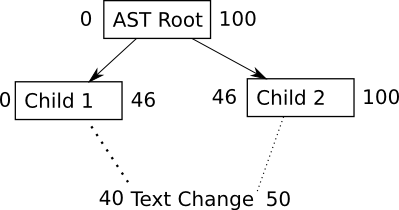
\includegraphics[scale=1]{DrilldownEx}
 \end{center}
 \caption{An AST showing a partial overlap between child 2 and a text change, and child 3 and a text change}
 \label{fig:troubleASTNode}
\end{figure}

Another interesting question is how the tool deals with situations where a text change partly overlaps an AST node or an AST node only partly covers a text item.  This issue is shown in Figure \ref{fig:troubleASTNode}. In the situation where only part of an AST Node contains the text change, the children of that AST Node are examined to see if they are fully within the text change.  If not it keeps recursively checking until either a child falls completely outside the change or is completely in the change.  

In the case where portions of a text change which are outside of a AST node then that change could be a comment or white space. This can be seen in both Figure \ref{fig:findingASTNode} and Figure \ref{fig:troubleASTNode} because in both of these portions of text are outside a text node.  These are of interest to us because these are instances where the text may have been changed but it has no impact on the behaviour of the program.  The most likely instances of this is when a comment has changed or if white space has been introduced in the middle of source code. Once the AST node for both revisions has been matched with the text change we can compare the AST nodes and their children to discover if they would behave in the same fashion. If they do behave in the same fashion it could indicate that the change is an ascetic one.

Another change we are interested in is if items have been moved.  We would notice this if there is a both insert and a delete for similar AST node types within the same scope.  If a method has been shifted within a class we would notice similar AST nodes, one being deleted at one location, the other being inserted at a different location.  This is another example of a text change that does not change the behaviour of the program.

%If we can keep track of renaming

If we find examples of text based changes that do not change the programs' behaviour we have an indication that we can reduce the amount of changes necessary to update another view. This in turn could indicate that we would have less merge conflicts by reducing the overall number of changes.

% In order to do this the source code needs to be divided into understandable
% sections. When each of these sections for each revising are compared it is
% possible to determine if a section has been moved.  This enhances what can
% be detected when examining the differences between two files.
% 

\section{What the tool does}
% answer what it does and how

By checking to see if an insert at one point is similar to a delete at another point it is possible to see if the code block has moved. In order to determine if the move is one that has no impact the matches are only counted if a match can be found within the same container.  Here, a container is an enclosing scope within the source code, such as a class. For example if a method has been shifted within the same class the program will still act the same.  If a method is moved from one class into an inner class there is no guarantee that they will be evaluated to determine if there is a suitable match.  If a method is shifted from one class to an inner class however the programs' behaviour could have changed.

\begin{figure}[!t]
\begin{lstlisting}
public class SampleMoveAndChange {

  public static void main(String[] args) {
    System.out.println(circleArea(3));
  }

  public static double triangleArea(double base, double height) {
    return base / 2 * height;
  }

  public static double cubeSurface(double length) {
    return 6 * squareArea(length);
  }

  public static double circleArea(double radius) {
    return Math.PI * squareArea(radius);

  }

  public static double squareArea(double num) {
    return num * num;
  }

}
\end{lstlisting}
\caption{The original source code before methods have been moved}
 \label{fig:orig}
\end{figure}

\begin{figure}[!t]
\begin{lstlisting}
public class SampleMoveAndChange {

  public static double triangleArea(double base, double height) {
    return base / 2 * height;
  }

  public static void main(String[] args) {
    System.out.println(circleArea(3));
  }

  public static double cubeSurface(double length) {
    return 6 * squareArea(length);
  }

  public static double squareArea(double num) {
    return num * num;
  }

  public static double circleArea(double radius) {
    return squareArea(radius) * Math.PI;

  }

}
\end{lstlisting}
\caption{The modified with methods that have both moved and have changed slightly}
 \label{fig:orig}
\end{figure}


To determine if blocks of code have been moved we need to find a deleted block of code that is most similar to an inserted block of code.  An example of this is if we have the original program shown in Figure ~\ref{fig:orig} and the modified program shown in Figure ~\ref{fig:modified}

\begin{figure}[!t]
\begin{center}
 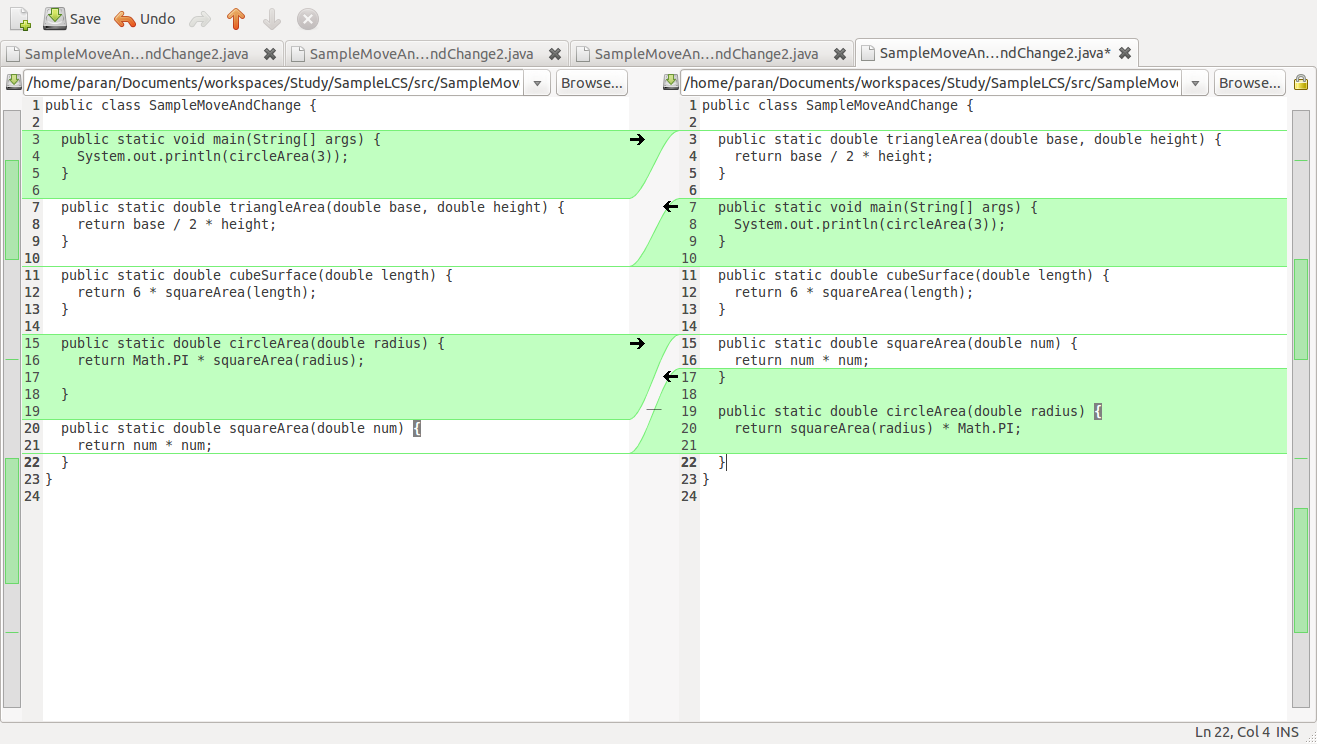
\includegraphics[scale=.3]{movediff}
 \end{center}
\caption{A comparison of similar code with methods that have moved and changed}
 \label{fig:orig}
\end{figure}


A comparison of the source code using a graphical merge tool is shown in Figure ~\ref{fig:modscreenshot}.  Because two methods have moved there are two deletions from the original and two insertions into modified version.  However the method that calculates the area for a circle has also changed slightly. In the Refactor Categories Tool all the Java are changes are represented by the AST for the original source code and the AST for the modified source code. We are not able to directly compare the AST nodes to see if they are equal because the \lstinline{circleArea} method has been changed slightly. By recursively comparing all the AST nodes for a delete candidate against all the AST nodes for a insert candidate we are able to calculate a score that shows how similar they are.  As in the example there could be multiple inserts and we need to compare them against multiple deletes to obtain all the scores.

To calculate the scores for a single change we start at the root AST node for both the insert and delete candidates.  If the root nodes are similar we can then check their children. By performing a diff between the lists of children for both the insert and delete candidates we obtain the minimum number of differences.  If an extra child AST node has been inserted or a child AST node is deleted then 1 is added to the score. If a child AST node has been modified it is the equivalent of both a child AST node being inserted and one being deleted so 2 is added to the score. If there has been no change to a child AST node we need to recursively assign a score using its children. To get the total percentage of children that changed we divide the score against the total number of children for both the delete and insert AST nodes we are scoring.

In the example in Figure ~\ref{fig:matchComp} two AST node are being compared with each other. The red AST node has been deleted and an orange AST node have been inserted. Because the yellow node has been modified it has effectively been deleted and a green node has been inserted. This means has been a total of 4 changes to this level of the AST. 

\begin{figure}[!t]
 \begin{center}
 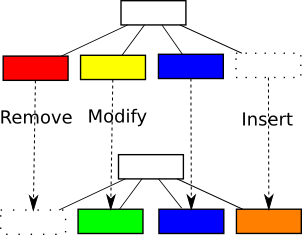
\includegraphics[scale=1]{matchComp}
 \end{center}
 \caption{Two AST nodes being compared to each other by comparing the differences in their child nodes.}
 \label{fig:matchComp}
\end{figure}

In addition to the comparison of AST nodes to test for where Java code has move we also need to determine when comments move.  As it is possible for the comment to change we also need to test for similarity.  This is done by comparing the characters in from the code block that has been deleted with characters from the code block that has been inserted.  A comparison is done between the two code blocks using a diff to obtain the smallest number of changes. A score of 1 is added for each deleted or inserted of a character.  If a character has been modified a score of 2 is added. To obtain the percentage of items changed the score is divided by the total number of characters in both code blocks.

Scores are stored in a two dimensional array where the rows are insert candidates and the columns are delete candidates.  We use the greedy algorithm to select the lowest score in the array.  Insert and delete candidate that are selected are recorded as a move and should not be compared with anything else. The comparisons that are no longer possible are in the same column or row in the array.  The comparisons that are no longer possible are removed and the next lowest score for a match is evaluated.  To ensure that anything cannot be matched with anything once all good matches are eliminated a limit is set ensuring that any further matches are ignored.  The two items that could have otherwise been matched will remain a solitary insert and a delete.

To a limited extent the Refactor Categories Tool can also deal with renaming. It does this by examining the node and seeing if its children have remained the same and its type remain the same but its name has changed. It can not analyse nodes where the name has not changed as these are not picked up by the initial text comparison.

The Refactor Categories Tool first does a cursory examination of the text differences between two files. It then examines both the differences in executable Java code and the differences between comments and white-space. 



\section{Performance}
 This means that performance is an issue especially for large software projects that have many changes. This means we have not only had to look at using more memory for the Refactor Categories Tool but also had to make some changes to the code to free up more memory where required.

\begin{description}
 \item [By setting object references back to null when they are no longer used.]
  Once a difference has been detected we attempt to remove any of the information we are not going to use in the future.  This should help the garbage collector free up memory. We do this by setting the AST nodes recorded against a difference to null once the difference has been discovered. 
\item [By not analysing AST node that did not have a text based change.] 
  By ignoring AST nodes and any of their child nodes that do not have a text based change comparing all the AST nodes can be avoided.  This will also help to speed up analysis as these nodes do not need to be analysed to see if they match.
\item [matching within only the required scope.]
  If we were not testing for moves in the same scope we would need to test every deleted AST node against every inserted AST node for the entire file. By stipulating that we can only be sure if it is a legal move if it is in the same scope we not only eliminate a lot of relocations of source code that are illegal but also reduce the number of items that need to be compared. In addition to this the AST node along with its type are recorded in a hash map.  This ensures that only AST nodes that are a similar type are compared against each other.
\end{description}

% future work: by keeping track of equivalences there is no need to retest
% using the AST

\section{Design decisions}
Java was chosen as both the language to write the tool in and to be the language that the tool would recognise.  This was done as it was a language we understood and to make use of JDime if it was going to be part of the tool.  We wanted to use git due to its distributed nature.  The reasons for choosing a distributed version control system was that we wanted each private view being able to function on its own as a fully fledged project without being dependant on a server.  As we were already using Java rather than using the main Git distribution which is written in C we needed to use JGit instead.

We could not use JDime because of the issues discussed earlier. Instead we used JastAddJ the same Java implementation that JDime uses so that we could implement some of the differences we required including being comment aware and only examining each of the copies of source code.

There are a number of design differences between JDime and the Refactor Categories Tool.  Instead of doing a text comparison first and only proceeding to analyse the program using an AST if there are conflicts the categorization tool examines all files that have a difference in them.  Although this takes longer and is more memory intensive there are some advantages to this. The main advantage is related to the concept of keeping branches as consistent as possible whenever there is a change. An example of this advantage is if a merge was done using an ordinary text comparison and there is a non functional change to only one revision. Examples of a non functional change could include reordering methods or inserting a comment.  As the changes were only done to one of the revisions there is no conflict and JDime only does a text based merge.  During this text based merge, in addition to any of the changes to functionality that we want, we get the non functional changes that change the source code without changing the programs' behaviour. By examining all changes irrespective of if the text has conflicts means that the Refactor Categories Tool can determine if it is a change that would not affect the behaviour of a program.

As there is a cost overhead with testing all the changes rather than just the conflicting ones the categorization tool needs to be efficient in how it tests changes.  Assuming that changes occur in select areas within the file there are portions of the file that have not been changed.  We have developed a method that spends a smaller amount time in  within the portions that have already been identified as not containing changes.  Like JDime we initially do a text based merge.  The text based merge we use however uses the histogram merge in JGit.  This allows us to use information from the text based merge when we analyse the AST tree.  The information used is the ranges of line numbers and operations identified by the histogram merge. The change set has been taken from the original JGit based diff contains the start and end of the change in both files and what type of change it is (insert delete or modify).  By reusing these ranges of line numbers it is possible to figure out which AST items these changes affect. This is done by loading the file into the JastAddJ parser to get an AST tree. Line numbers for each item in the tree are then compared to line numbers from the change set. The line numbers are matched to the position information stored in each AST node using the following method.

The root of the AST is identified as the AST node we need to start at. 
We only begin any analysis, if the AST node resides completely within a block of text changes.
If there are any separate blocks of changes that occur between the start position of the AST node and the end position of the AST node then we recursively examine the AST nodes children.

% The Refactor Categories Tool first works out which text has changed using 
% the same method as JGit.
% This initial examination returns the differences based on a line by line 
% basis rather than using a smaller granularity.
% This means that the set of changes found could still contain code that is 
% comparatively the same.
% The set of changes found in using the JGit histogram comparison are then 
% evaluated.
% The reason for this is that some items of text could be in a differing order 
% but still be a valid Java program
% 
% 
% In order to resolve some limitations with JDime and the text only merge in 
% GIT information about which line numbers are retained after the first text 
% merge.  In JDime these are ignored and the AST is relied upon to hold all 
% the information.


% after finished drill down we have a record of the same changes as JGit
% except now we also have the ASTs

In some instances there is no position information stored in the JastAddJ AST nodes.  This could be because they are generated by the parser to reflect parts of the Java language that are inferred rather than directly mentioned in the code.  An example of this would be the use of super in the constructor.  Even if it is not written in the code for every constructor has a super. Likewise all methods mentioned in an interface have a public type even if is not in the code.

To get around this problem we have needed to discover the end position of the previous AST Node to determine the position the inferred AST node should occupy.  This means that the inferred AST node is in the right position but is not represented by a block of text in the source code. 

Comment and white-space are also examined separately as they also could give some indication of where code has been moved from or to.
Before being checked to find matches unnecessary white-space is identified and recorded.
Any text that remains is examined to determine if its is a comment. 

Because of the way we are using the position in the code to identify AST nodes there are circumstances when parts of the Java programming language are identified as being surplus text. These have already been identified and represented as an AST Node. By identifying comments we can eliminate any of the items falsely recorded as comments.

% Comments and white-space cannot be shown in the AST tree so they need to be
% dealt with separately

% comparing AST nodes
% the matcher and how using a score works
% finding the best match
% 
% 
% explain how we limit matching just to the parent of the thing being matched

Rather than comparing everything with each other to determine matches it is more efficient to match just the items that are under the same AST structure.  This means that it is more likely that we get a match that is going to be relevant and valid.  An example of this is matching methods. If the methods are under the same container (a class) they may be legally swapped without causing issues.  If the method has been moved to an inner class from an outer one however it becomes more complicated and we cannot guarantee that the code is equivalent.  


\section{Limitations of the tool}
The Refactor Categories Tool focuses only on areas where there has been a text change in the source code. 
It is harder to investigate any change that has causes side effects in unchanged code.  Fortunately it is not often that this type of side effect will be purposely placed in the code as it reflects bad design decisions.  This may however be an issue with bugs, which are unintentionally occur in the code.
This also means that the Refactor Categories Tool will not be able to tell when some code has been copied but the original remains unchanged. Instead it will assume that it is a completely new insertion of code.

If a change of a variable name is noticed the program still retains the same behaviour if the rename operation has worked on all instances where the old name was previously used.  As we do not examine parts of the code that have not experienced a text based change we cannot guarantee that a rename operation is a valid one. We have an indication that it might be if the code still compiles without error. If a variable name is changed to that of an already existing variable however the behaviour of the program could change. This is known as a \emph{semantic conflict}.  This issue already exists in a text based merge and Fan \cite{Fan2012}, Shao \cite{Shao2009} and others address this issue. 
